% Skill Without Physics — full submission draft.
% Compiled with article class in two-column ICML-like layout; swapping in an
% official conference style file (e.g. icml2027.sty) requires only replacing
% the preamble block marked STYLE.
\documentclass[10pt,twocolumn]{article}

% ---------- STYLE (replace with conference style for submission) ----------
\usepackage[margin=0.9in,columnsep=0.25in]{geometry}
\usepackage{times}
\usepackage[T1]{fontenc}
\usepackage[utf8]{inputenc}
% --------------------------------------------------------------------------
\usepackage{amsmath,amssymb}
\usepackage{booktabs}
\usepackage{graphicx}
\usepackage{microtype}
\usepackage{xcolor}
\usepackage[hidelinks]{hyperref}
\usepackage{caption}
\captionsetup{font=small,labelfont=bf}
\usepackage{longtable}
\usepackage{natbib}

\newcommand{\Mone}{\mathrm{M1}}
\newcommand{\Mtwo}{\mathrm{M2}}
\newcommand{\Mthree}{\mathrm{M3}}
\newcommand{\uw}{\overline{u'\omega'}}
\newcommand{\vw}{\overline{v'\omega'}}

\title{Skill Without Physics: A Mechanistic Audit of\\ Neural Gravity-Wave Parameterizations}
\author{Anonymous Authors\\ \small Draft v3.1 --- every number traceable to a stamped results file in the released repository}
\date{}

\begin{document}
\maketitle

\begin{abstract}
Neural-network parameterizations of atmospheric gravity-wave (GW) momentum fluxes increasingly inform climate-model development, and horizontal nonlocality is credited for much of their skill. We present the first mechanistic interpretability study of a parameterization emulator, auditing the released single-column / $3{\times}3$-stencil / Attention-U-Net hierarchy of Gupta et al.\ (2025) with a pre-registered hypothesis funnel: 30 hypotheses generated, 24 screened (15 killed), 1 measured, 5 deferred with reasons, and 1 further killed at held-out confirmation. Three findings emerge. (1)~The U-Net's variance and extreme-tail calibration rides substantially on a \emph{position-indexed prior}: convolutional padding lets the network infer absolute position, and rolling the input map---which changes no physics---collapses its flux-variance calibration from 1.10 to 0.33. Roll ensembles attribute up to 62\% of variance calibration and 37\% of extreme-tail (P99.9) calibration to position (an upper bound), while bulk-quantile calibration is flow-driven; the calibration split replicates on a second held-out month. Notably, pooled-histogram Hellinger distance---the literature's headline distributional metric---is insensitive to this collapse and can even be \emph{improved} by physically absurd variance inflation; quantile-ratio ladders discriminate. (2)~The U-Net's causally used context is long-range (median 4 grid cells, ${\sim}1200$\,km at T42) but isotropic and unaligned with ray-traced propagation directions. (3)~Under single-aspect grafts of real columns---a protocol whose amplitude family is validated without conditions on a 1D testbed emulator that demonstrably learned its physics (response tracking 0.94 there vs.\ 0.49 here)---the column models show no filtering response at typical columns, drag that ignores wind rotation, and non-monotone amplitude response. These surrogates achieve much of their offline skill as regime pattern-matchers with geographic priors rather than by encoding wave physics, with direct implications for out-of-distribution trust and for how distributional skill should be measured.
\end{abstract}

\section{Introduction}\label{sec:intro}

Atmospheric gravity waves transport momentum from their sources---mountains, convection, jets and fronts---into the middle atmosphere, where their breaking drives circulations that climate models cannot resolve and must parameterize \citep{fritts2003}. Hand-built GW parameterizations embody strong simplifying assumptions (single-column propagation, steady launch spectra), and a growing literature replaces them with neural networks trained on high-resolution data \citep{espinosa2022,hardiman2023,gupta2024ml,gupta2025}. A headline result of this line is that \emph{horizontal nonlocality}---giving the network a view of neighboring columns or the whole domain---substantially improves offline skill, with the natural and widely voiced hope that networks so equipped learn genuinely nonlocal wave physics such as lateral propagation.

Whether that hope is warranted is a question about \emph{mechanism}. The tools of mechanistic interpretability---probing with controls, activation patching, controlled input interventions, representation analysis---are built for such questions, yet have barely touched scientific surrogates: prior interpretability of GW emulators stops at kernel Fourier analysis \citep{pahlavan2024}, gradient receptive fields \citep{pahlavan2025}, and SHAP attributions \citep{haslauer2026}. To our knowledge (verified by a systematic scan, August 2026), no activation-level or interventional study existed for any subgrid parameterization emulator.

We conduct such a study on the \emph{actual released artifacts} of \citet{gupta2025}: the hierarchy $\Mone$ (single-column MLP), $\Mtwo$ ($3{\times}3$ stencil), $\Mthree$ (Attention U-Net), the released checkpoints, and held-out months of the models' test year. Because interpretability is vulnerable to cherry-picking, the entire investigation is organized as a pre-registered hypothesis funnel (Sec.~\ref{sec:method}): falsifiable statements and kill criteria fixed before each test, adversarial critic passes at stage gates, held-out-month confirmation for surviving claims, and full reporting of all outcomes (Appendix~\ref{app:funnel}). Fifteen of 24 screened hypotheses died---including our own pre-registered flagship (``the U-Net's influence pattern follows wave-propagation geometry''; it does not)---and the surviving findings were in several cases discovered \emph{by} the kills.

\textbf{Contributions.}
\begin{enumerate}\itemsep2pt
\item \textbf{A position-indexed variance prior} (Sec.~\ref{sec:pos}). $\Mthree$ infers absolute position through zero-padding and uses it as a de facto geography channel: its distinguishing skill---variance/extreme-tail calibration---collapses under longitude rolling (variance ratio $1.10\!\to\!0.33$), with up to 62\% of variance calibration attributable to position, localized causally to the bottleneck (${\sim}48\%$) and decoder (${\sim}39\%$), concentrated over climatological hotspots, replicated on a second month, and visible as a $+5\%$ error seam at the map boundary.
\item \textbf{The character of the learned nonlocality} (Sec.~\ref{sec:nonlocal}). Causal occlusion shows context is used to a median radius of 4 cells (${\sim}1200$\,km), yet influence maps are isotropic (median axis ratio 1.07) and unaligned with ray-traced propagation; the $3{\times}3$ gain is carried by the full multivariate neighborhood pattern---not by gradients, single directions, linear readouts, or any low-rank channel we could identify.
\item \textbf{A positive-controlled physics-trust audit} (Sec.~\ref{sec:audit}). Under single-aspect grafts of real columns the models show no critical-level filtering at typical columns, wind-rotation-blind drag, and non-monotone amplitude scaling---while a testbed emulator that provably learned its (1D) physics passes the same battery.
\item \textbf{Methods findings} (Secs.~\ref{sec:hellinger},~\ref{sec:setting}): pooled Hellinger distance is insensitive to---and gameable against---exactly the failure it is used to detect; and a reproducibility hazard in the public data stack (normalization-incompatible public data + checkpoints; $R^2$ of $-4$ to $-81$ without our released conversion).
\end{enumerate}

This is an offline study of one released family at T42; Sec.~\ref{sec:limits} details scope limits, including why some nulls may be resolution-conditional.

\section{Related Work}\label{sec:related}

\textbf{ML parameterization of GWs.} Scheme emulation established feasibility and out-of-sample generalization \citep{espinosa2022,hardiman2023}; reanalysis-driven flux prediction introduced the nonlocality hierarchy audited here \citep{gupta2024ml,gupta2025}, trained on Helmholtz-decomposed ERA5 fluxes \citep{gupta2024data} and evaluated with Hellinger distances; foundation-model fine-tuning followed \citep{gupta2025prithvi}. Nonlocal inputs for subgrid closures more broadly: \citet{wang2022}.

\textbf{Interpretability of scientific ML.} GW-specific prior art is weight- or attribution-level \citep{pahlavan2024,pahlavan2025,haslauer2026}. Mechanistic tools recently reached weather foundation models---SAEs and steering on GraphCast \citep{macmillan2025}, probes on Aurora \citep{richards2025}, SAEs on Walrus \citep{rosenfeld2026}, cross-model CKA \citep{craig2026}---but no probing, patching, or interventional study of a parameterization emulator preceded this work.

\textbf{CNN position encoding.} Padding leaks absolute position into CNNs \citep{islam2020,kayhan2020}. Its consequences for scientific surrogates---a memorized geographic prior doing work attributed to physics---were unmeasured; we quantify them causally.

\section{Setting: Models, Data, and a Reproducibility Hazard}\label{sec:setting}

\subsection{The released hierarchy}\label{sec:models}
Inputs are ERA5-derived columns on a T42 Gaussian grid ($64\times128$), 122 model levels (surface to ${\sim}45$\,km): $u,v,\theta$ (optionally $w$), plus scalars $[\mathrm{lat},\mathrm{lon},z_s]$ for $\Mone/\Mtwo$; outputs are both GW momentum-flux components at all levels (244 channels). Outputs are cube-root transformed and globally standardized,
\begin{equation}\label{eq:norm}
\tilde F \;=\; \big((F-\mu_F)/\sigma_F\big)^{1/3},\qquad
\tilde u \;=\; (u-\mu_u)/(3\sigma_u),
\end{equation}
with fixed global constants. $\Mone$ is a 6-hidden-layer MLP ($\mathrm{hdim}=4\times\mathrm{idim}$, LeakyReLU) on single columns; $\Mtwo$ prepends one $3{\times}3$ valid convolution; $\Mthree$ is an attention-gated U-Net (additive skip \emph{gating}, not self-attention; encoder $64\!\to\!1024$ channels over four poolings) on the global map, and---consequentially---\emph{omits} the lat/lon/$z_s$ scalars from its inputs. Training used 2010/2012/2014 (all months); all of 2015 is test (from the released training script). We use July 2015 (screening), January 2015 (confirmation; analyses restricted to a four-entry ledger pre-registered before the file was opened), and two released August snapshots. One checkpoint per configuration exists; no seed ensembles were released. Two code-level facts matter later: the checkpoints carry vestigial, never-executed BatchNorm parameters (all $\texttt{num\_batches\_tracked}=0$), and $\Mthree$'s convolutions zero-pad a longitudinally \emph{periodic} domain.

\subsection{A reproducibility hazard}\label{sec:hazard}
The anchor's training-format monthly files are published in WxC-Bench. All of them share one \emph{alternative} normalization---different constants and a $1\times\!\sigma$ (not $3\times\!\sigma$) $u,v$ convention---despite metadata identical in wording to the author-released test files. Fed to the released checkpoints as-is they yield $R^2$ of $-57$ to $-81$ ($\Mone$) and $-4.1$ to $-4.4$ ($\Mthree$). We derived the exact affine conversion and validated it three ways: algebraic round-trip; a \emph{consecutive-hour test} (the July file's last hour is adjacent to the released August snapshot's first hour; converted fields match with regression slopes ${\approx}1$); and a skill gate (converted data reproduces paper-consistent $R^2$, e.g.\ $\Mthree$ 0.37--0.42 in both months). All experiments auto-detect and convert; utilities are released.

\subsection{Replication gate}\label{sec:replication}
Table~\ref{tab:replication} replicates the anchor's core offline result on both held-out months: RMSE and Hellinger orderings $\Mthree{<}\Mtwo{<}\Mone$ (robust to $\cos\varphi$ area weighting), with $\Mthree$ beating $\Mtwo$ in \emph{744/744} paired timesteps in each month. The skill benefit of nonlocality is unambiguous; this paper asks what implements it.

\begin{table}[t]\centering\small
\caption{Full-month replication on held-out data (744 hourly timesteps per month). RMSE in normalized space; Hellinger $H$ and variance ratio $\sigma^2_{\hat F}/\sigma^2_F$ in physical space. Source: \texttt{results/a4\_fullmonth}, \texttt{a4\_january}.}
\label{tab:replication}
\resizebox{\columnwidth}{!}{\begin{tabular}{llccccc}
\toprule
Month & Model & RMSE & RMSE$_{\cos\varphi}$ & $H_{uw}$ & $H_{vw}$ & $\sigma^2$-ratio \\
\midrule
July 2015 & M1 & 0.7844 & 0.7882 & 0.0644 & 0.1264 & 0.360 \\
 & M2 & 0.6980 & 0.6958 & 0.0493 & 0.0970 & 0.363 \\
 & M3 & 0.6775 & 0.6764 & 0.0399 & 0.0433 & 1.066 \\
\multicolumn{7}{l}{\quad\footnotesize paired M2$-$M3 RMSE: mean 0.0204, 95\% CI [0.0202, 0.0207]; M3 better in 100\% of 744 timesteps} \\[2pt]
January 2015 & M1 & 0.7444 & 0.7705 & 0.0699 & 0.1080 & 0.419 \\
 & M2 & 0.6653 & 0.6809 & 0.0502 & 0.0914 & 0.351 \\
 & M3 & 0.6500 & 0.6661 & 0.0414 & 0.0461 & 0.996 \\
\multicolumn{7}{l}{\quad\footnotesize paired M2$-$M3 RMSE: mean 0.0152, 95\% CI [0.0150, 0.0155]; M3 better in 100\% of 744 timesteps} \\[2pt]
\bottomrule
\end{tabular}
}
\end{table}

\section{A Pre-Registered Audit}\label{sec:method}

\textbf{Funnel.} Thirty falsifiable hypotheses across seven families (information content, representations, architecture, gates, transfer, failure structure, physics consistency), each with technique family, cheapest test, and kill criterion; an adversarial critic pass hardened thresholds and controls before screening. Screening tests were budgeted ${<}20$ minutes of CPU; survivors advanced to deep dives under pre-registered analysis plans; January confirmations were limited to the pre-registered ledger. Deviations were logged when they occurred (all appear in the released log). \textbf{Multiple comparisons:} every test is reported (Appendix~\ref{app:funnel}); verdicts are pre-registered thresholds, not $p$-values; the funnel table is the full family of outcomes.

\textbf{Distributional metrics.} For flux component $F$ with prediction $\hat F$ (physical units), the \emph{quantile-ratio ladder} is
\begin{equation}\label{eq:ladder}
R_q \;=\; \frac{Q_q(|\hat F|)}{Q_q(|F|)},\qquad q\in\{0.9,\,0.99,\,0.999\},
\end{equation}
computed per timestep and summarized by mean with a 2000-resample bootstrap CI over timesteps. Pooled Hellinger uses $H = 1-\sum_i\sqrt{p_i q_i}$ on common histograms. Variance ratio is $\mathrm{Var}(\hat F)/\mathrm{Var}(F)$ pooled over the month.

\textbf{Interventions.} (i) \emph{Longitude roll}: $T_r$ shifts the input map $r$ cells (physics-neutral: the domain is periodic; $\Mone$ is roll-invariant, $\Mtwo$ roll-equivariant---both are controls). Predictions are unrolled before scoring; the \emph{position share} of a calibration quantity $V$ is
\begin{equation}\label{eq:share}
S_V \;=\; \big(V_{0} - \textstyle\frac{1}{15}\sum_{r} V_{r}\big)\,/\,V_{0},\quad r\in\{8,16,\dots,120\},
\end{equation}
an \emph{upper bound} on position dependence (rolling also moves inputs off-manifold). (ii) \emph{Cumulative roll-patching}: encoder activations from the unrolled forward are roll-aligned and patched into the rolled forward at sites $\mathrm{conv}1..k$; an identity control (patching a run with its own activations) reproduces the base prediction to machine precision. (iii) \emph{Occlusion}: inputs outside radius $r$ of a target column are replaced by monthly climatology; the saturation radius is the smallest $r$ with target-column MSE within $5\%$ of the full-input value. (iv) \emph{Neighborhood clamping/resampling} for $\Mtwo$.

\textbf{Physics grafts.} Single-aspect modifications of real columns under an admissibility rule ($\max_c |(x_c-\mu_c)/\sigma_c|\le 4$ against monthly column statistics): \emph{reflection} creates a directional wind reversal above level $z_c$,
\begin{equation}\label{eq:graft}
u'(z) = u(z) + \beta\,\big(2u(z_c)-2u(z)\big),\quad z\ \text{above}\ z_c,
\end{equation}
with per-column maximal admissible dose $\beta\in[0.25,1]$; \emph{amplitude} scales deviations from climatology by $a\in[0.25,1.5]$; \emph{rotation} rotates $(u,v)$ jointly by $\phi$. Responses: suppression $s = 1 - \langle|\hat F'|\rangle_{\text{above}}/\langle|\hat F|\rangle_{\text{above}}$; Spearman $\rho$ of response vs.\ $a$; circular alignment of drag-vector rotation with $\phi$.

\textbf{Positive control.} Nulls are meaningful only if the tests detect physics where it exists. We ran the same graft families on the released \texttt{qbo1d} testbed emulator (10-layer MLP), whose stochastic 20-wave source physics is exactly computable, giving ground truth $\mathbb{E}[S|u]$ by Monte Carlo (200 draws). The emulator is faithful (median corr.\ 0.983 to $\mathbb{E}[S|u]$); the \emph{amplitude family validates unconditionally} (median Spearman 0.94 between emulator and true response curves) and is the load-bearing null; the reflection family validates where the true effect is detectable (median corr.\ 0.75 at relative effect $\ge$10\%; agreement rises with effect size, $r=0.93$)---a conditioning that cannot be applied in ERA5, where ground truth is unknown (Sec.~\ref{sec:limits}).

\textbf{Probing.} Ridge probes with mandatory controls: random-init network of identical architecture, raw-input baseline, shuffled labels, and spatial train/test splits (disjoint longitude sectors); we report \emph{selectivity} $=$ metric(real) $-$ $\max$(metric(rand-init), metric(input)).

\section{Results}\label{sec:results}

\subsection{Where the distributional skill lives}\label{sec:ladder}
Table~\ref{tab:ladder} and Fig.~\ref{fig:ladder} give the calibration ladders. All models compress typical amplitudes severely (July P90 ratios 0.07/0.11/0.28 for $\Mone/\Mtwo/\Mthree$); calibration improves with quantile level and with nonlocality until $\Mthree$'s extreme tail is calibrated (P99.9 $=1.02$, CI $[1.005,1.043]$). January replicates the pattern in full ($\Mthree$: 0.32/0.77/1.04). Month-scale variance ratios split the hierarchy sharply: $0.36/0.36/1.07$ (July), $0.42/0.35/1.00$ (January). \emph{The U-Net's distinguishing skill is variance/tail calibration.}

\begin{figure}[t]\centering
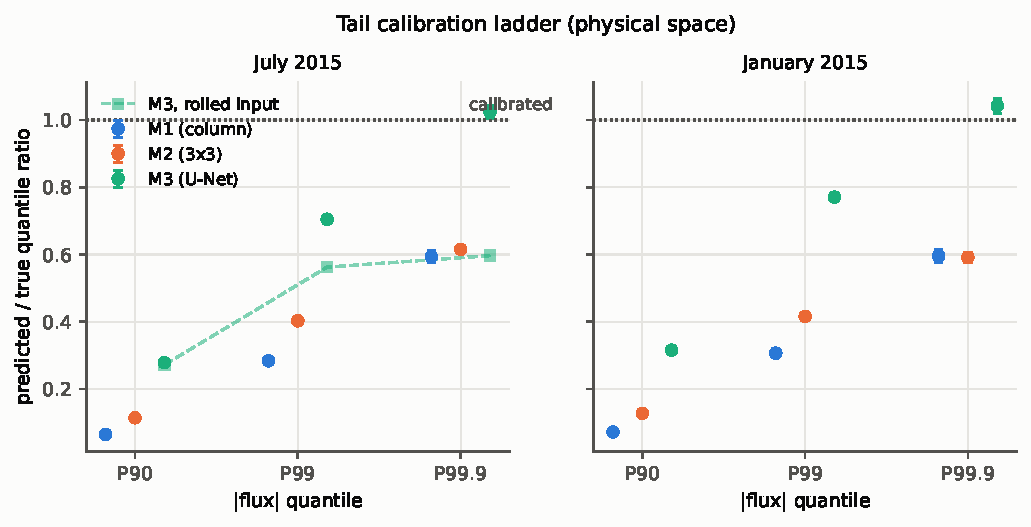
\includegraphics[width=\columnwidth]{figures/fig2_calibration_ladder.pdf}
\caption{Quantile-ratio calibration ladders (Eq.~\ref{eq:ladder}; physical space; bootstrap 95\% CIs over timesteps). Left: July, including $\Mthree$ under a 64-cell input roll---its extreme-tail calibration collapses to the column-model band. Right: January replication. Sources: \texttt{screen\_a5\_tails}, \texttt{j1\_tails\_january}, \texttt{gateweek\_g2}.}
\label{fig:ladder}
\end{figure}

\begin{table}[t]\centering\small
\caption{Calibration ladders $R_q$ with bootstrap 95\% CIs.}
\label{tab:ladder}
\resizebox{\columnwidth}{!}{\begin{tabular}{lccc}
\toprule
 & P90 & P99 & P99.9 \\
\midrule
\multicolumn{4}{l}{\emph{July 2015}} \\
M1 & 0.065 [0.064, 0.066] & 0.284 [0.272, 0.297] & 0.593 [0.576, 0.611] \\
M2 & 0.114 [0.112, 0.116] & 0.403 [0.394, 0.412] & 0.615 [0.605, 0.626] \\
M3 & 0.278 [0.274, 0.283] & 0.705 [0.693, 0.716] & 1.024 [1.005, 1.043] \\
M3 (rolled 64) & 0.272 [0.263, 0.279] & 0.563 [0.533, 0.586] & 0.597 [0.547, 0.638] \\
\addlinespace\multicolumn{4}{l}{\emph{January 2015}} \\
M1 & 0.072 [0.070, 0.074] & 0.307 [0.294, 0.319] & 0.595 [0.577, 0.614] \\
M2 & 0.128 [0.125, 0.130] & 0.416 [0.408, 0.423] & 0.591 [0.577, 0.605] \\
M3 & 0.316 [0.310, 0.321] & 0.771 [0.758, 0.783] & 1.042 [1.020, 1.063] \\
\bottomrule
\end{tabular}
}
\end{table}

\subsection{Finding 1: a position-indexed variance prior}\label{sec:pos}

$\Mthree$ receives no coordinates or orography, yet three causal probes show it knows where it is---and that its calibration advantage depends on it.

\textbf{Roll test and decomposition.} Under $T_{64}$, $\Mthree$ degrades globally ($+15\%$ RMSE) and its variance calibration collapses to $0.33$---\emph{below} $\Mtwo$---with P99.9 falling $1.01\!\to\!0.60$, while pooled Hellinger is unchanged ($0.0745\!\to\!0.0744$). The 15-roll ensemble (Fig.~\ref{fig:roll}, Table~\ref{tab:roll}) yields a symmetric distance curve (0.54 at $r{=}8$, minimum ${\sim}0.33$ at half-domain, recovering to 0.56 near full circle---an internal falsification check that passes) and position shares (Eq.~\ref{eq:share}) of 62\% (variance), 37\% (P99.9), 17\% (P99), 2.5\% (P90): \emph{the position prior supplies extreme-tail variance specifically; bulk calibration is flow-driven}. Regionally, the base variance ratio is $1.29$ over the eight climatological hotspot boxes vs.\ $1.02$ elsewhere, collapsing to $0.24/0.37$ under roll: the prior lives where the hotspots are.

\begin{figure}[t]\centering
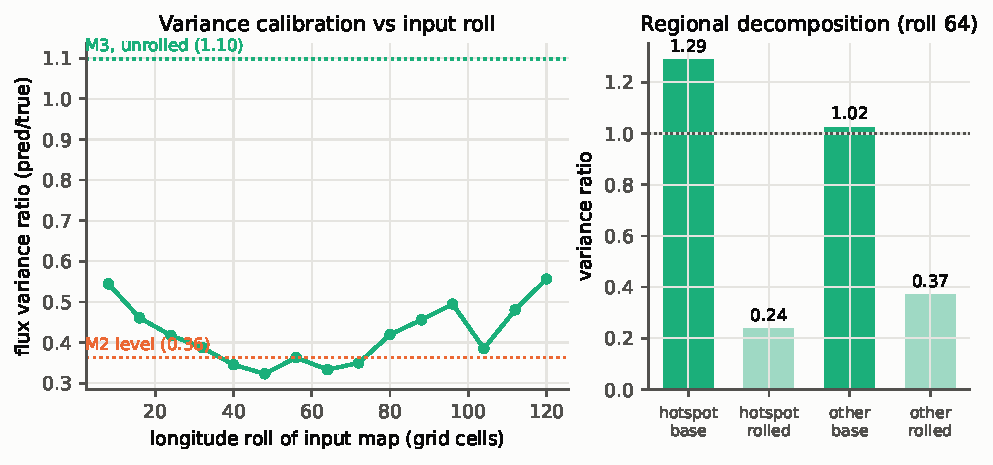
\includegraphics[width=\columnwidth]{figures/fig3_roll_position_prior.pdf}
\caption{Left: $\Mthree$ variance ratio vs.\ input roll distance (12 eval timesteps per roll); symmetry about the half-domain and recovery near the full period tie the collapse to \emph{position}, not to generic input perturbation. Right: regional decomposition at roll 64. Source: \texttt{d1\_rollensemble}.}
\label{fig:roll}
\end{figure}

\begin{table}[t]\centering\small
\caption{Roll-ensemble decomposition and causal localization.}
\label{tab:roll}
\resizebox{\columnwidth}{!}{\begin{tabular}{lccc}
\toprule
Quantity & Unrolled & Roll ensemble (15 rolls) & Position share (upper bd.) \\
\midrule
$\sigma^2$-ratio & 1.098 & 0.421 $\pm$ 0.073 & 62\% \\
P90 & 0.280 & 0.273 $\pm$ 0.004 & 2\% \\
P99 & 0.697 & 0.576 $\pm$ 0.017 & 17\% \\
P99.9 & 1.010 & 0.641 $\pm$ 0.047 & 37\% \\
\midrule
\multicolumn{4}{l}{\footnotesize Cumulative roll-patch restoration of $\sigma^2$-ratio: conv1--3 $\leq$1\%, conv4 12\%, conv5 61\%, decoder (residual) $\approx$39\%}\\
\bottomrule
\end{tabular}
}
\end{table}

\textbf{Causal localization.} Cumulative roll-patching restores essentially none of the calibration through encoder stages 1--3 ($-0.0/-0.0/-0.9\%$), $+12\%$ at conv4 and $+61\%$ cumulative at the bottleneck (Fig.~\ref{fig:rollpatch}); the residual ${\sim}39\%$ returns only when the decoder also sees consistent features. The identity control is exact (max deviation $0.0$), so this is not implementation error: \emph{the position computation forms where receptive fields become global and is applied again through decoder-stage boundary effects}, consistent with depth-accumulating padding information \citep{islam2020}. (Our pre-registered sanity endpoint wrongly assumed full encoder patching restores ${\approx}100\%$; the measured 61\% is a finding---the decoder itself computes position-sensitively---and the corrected assumption is logged.)

\begin{figure}[t]\centering
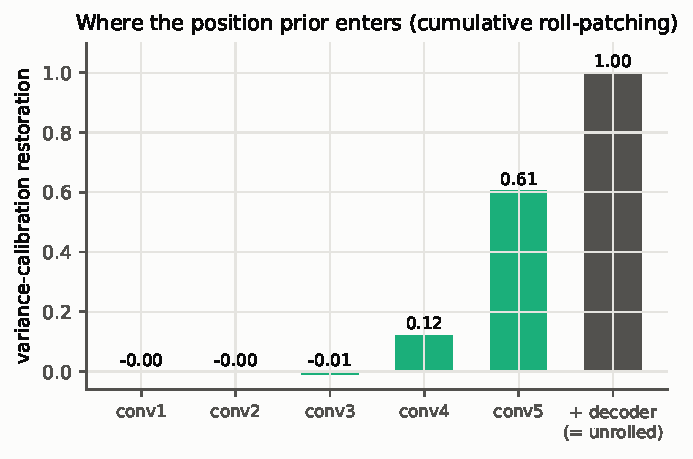
\includegraphics[width=0.95\columnwidth]{figures/fig5_rollpatch_localization.pdf}
\caption{Cumulative roll-patching: fraction of variance calibration restored when encoder activations up to a given stage are replaced by roll-aligned unrolled activations. Source: \texttt{d1\_rollpatch}.}
\label{fig:rollpatch}
\end{figure}

\textbf{The seam.} A visible corollary (Fig.~\ref{fig:seam}): $\Mthree$ alone carries $+5.1\%$ (July) / $+5.05\%$ (January) excess error at the three columns adjacent to the map boundary ($\Mone$: $-1.3\%$, $\Mtwo$: $-0.8\%$); under rolling the absolute excess moves with the padding boundary.

\begin{figure}[t]\centering
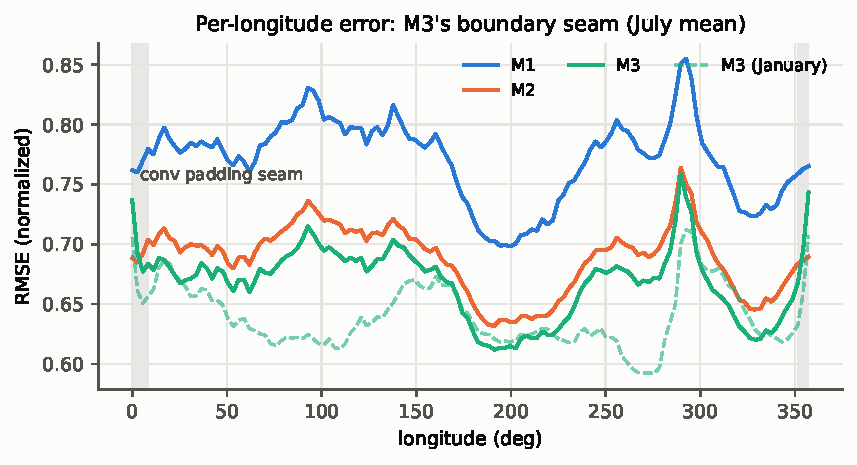
\includegraphics[width=\columnwidth]{figures/fig4_seam_profile.pdf}
\caption{Month-mean RMSE by longitude. Only the padded model ($\Mthree$) exhibits the boundary seam (shaded); the January overlay replicates it. Sources: \texttt{screen\_p4\_seam}, \texttt{a4\_january}.}
\label{fig:seam}
\end{figure}

\textbf{Not reconstruction; not rescaling.} Probes for $z_s$ from $\Mthree$'s first encoder stage read \emph{worse} than raw inputs ($R^2$ 0.06 vs.\ 0.45; random-init 0.08): the encoder \emph{discards} linearly readable orography rather than reconstructing it, and what little $z_s$ information exists at that depth is flow-derived, not position-derived (roll-arm probe: $R^2$ 0.14 vs.\ source geography, $-0.03$ vs.\ map position). Nor is the calibration a trivial output rescaling: per-channel variance-matching gains on $\Mtwo$ explode physical tails (P99 ratio 3.19; variance 11.9; RMSE 1.14) instead of reproducing $\Mthree$'s ladder.

\subsection{Finding 2: what the nonlocality is---and is not}\label{sec:nonlocal}

\textbf{Causally long-range.} Occlusion gives a median saturation radius of 4 cells (${\sim}1200$\,km at T42; $>16$ cells for 4/20 targets). $\Mtwo$'s context is information, not smoothing: clamping its neighborhood to nine copies of the center column makes it \emph{worse than} $\Mone$ (gap recovery $-0.70$; consistent across 24 timesteps).

\textbf{Not propagation-shaped.} Our pre-registered flagship---that influence maps $I(x,y)=\sum_c |\partial E/\partial x_c(x,y)|$ (with $E$ the predicted flux energy at a hotspot target) would be anisotropic along ray-traced propagation directions from our unit-tested tracer---was killed: median ring axis ratio 1.07 (threshold 1.3), wind alignment 9/20 (chance ${\approx}6.7/20$). At T42 the physically expected horizontal group displacements are largely sub-cell (Sec.~\ref{sec:limits}), but the widely voiced ``learned lateral propagation'' narrative finds no support at the scale where these models operate.

\textbf{Not simple.} The $\Mone{\to}\Mtwo$ gap is closed by neither a linear model on the stencil ($-47\%$ of the gap---worse than $\Mone$) nor gradient features ($+9.6\%$; 3 seeds); per-neighbor resample-ablation shows no wind-conditioned directional structure above threshold (octant spread/mean 0.165 $<$ 0.20; an upstream-biased hint at best); and the context signal at the last hidden layer is high-rank (top-5 PCs $=23\%$ of clamp-delta variance; projecting them out moves predictions 2.8\% toward $\Mone$). The neighborhood is consumed as a full multivariate pattern.

\textbf{Regime correlation (descriptive) and gates.} The $\Mtwo{\to}\Mthree$ gain concentrates in high-shear regions in both months (top-decile shear columns carry $2.9\times$/$1.8\times$ their share) and avoids steep orography ($0.27$/$-0.73$), but the pre-registered confirmation threshold ($\ge 2.0$) failed in January; we report the pattern descriptively. The attention gates are causally live (flattening the finest gate costs $+4.3\%$ RMSE, decaying monotonically with scale: $+1.4/+0.3/+0.1\%$) yet uncorrelated with instantaneous flux ($r=-0.015$ vs.\ nulls up to $0.07$): modulation, not source selection. Mid-encoder features do carry a regime code that transfers across disjoint regions (orographic-vs-nonorographic AUC 0.72; random-init control 0.40; entire shuffled-label range below 0.54).

\subsection{Finding 3: the physics-trust audit}\label{sec:audit}

Table~\ref{tab:grafts} and Fig.~\ref{fig:grafts} summarize the graft battery against the positive control.

\begin{table}[t]\centering\small
\caption{Physics-graft battery. ``Suppr.'' is flux suppression above the grafted reversal (Eq.~\ref{eq:graft}); $\rho$ is Spearman of response vs.\ amplitude; ``align.'' is circular alignment of drag rotation with wind rotation. OOD exclusions per arm are reported in the repository (e.g., rotation: 145--159 of 280--320 rotations excluded).}
\label{tab:grafts}
\resizebox{\columnwidth}{!}{\begin{tabular}{lccc}
\toprule
Arm & Median response & IQR & N \\
\midrule
\emph{Positive control (qbo1d emulator; ground truth known)} &  &  &  \\
Amplitude family (uncond.) & $\rho$ = 0.94 & [0.77, 0.94] & n=100 \\
Reflection (effect $\geq$ 10\%) & $r$ = 0.75 & [0.10, 0.83] & n=56 \\
\addlinespace\emph{Column models (ERA5)} &  &  &  \\
M1 reflection, Jul (uvtheta) & suppr.\ -0.008 & [-0.25, 0.26] & n=289 \\
M1 reflection, Aug (uvthetaw) & suppr.\ 0.043 & [-0.07, 0.30] & n=284 \\
M1 amplitude (uvtheta / uvthetaw) & $\rho$ = 0.49 / 0.49 & -- & n=162/136 \\
M1 wind rotation (uvtheta / uvthetaw) & align.\ 0.22 / 0.23 & -- & n=135/121 \\
\addlinespace\emph{Hotspot-center patch grafts (January)} &  &  &  \\
M3 patch (max dose) & suppr.\ 0.125 & [0.05, 0.16] & n=28 \\
\quad dose direction & 16/28 monotone, 12/28 anti &  & med.\ $\beta$=0.40 \\
M1 paired (max dose) & suppr.\ 0.092 &  & 22/28 monotone \\
\bottomrule
\end{tabular}
}
\end{table}

\begin{figure}[t]\centering
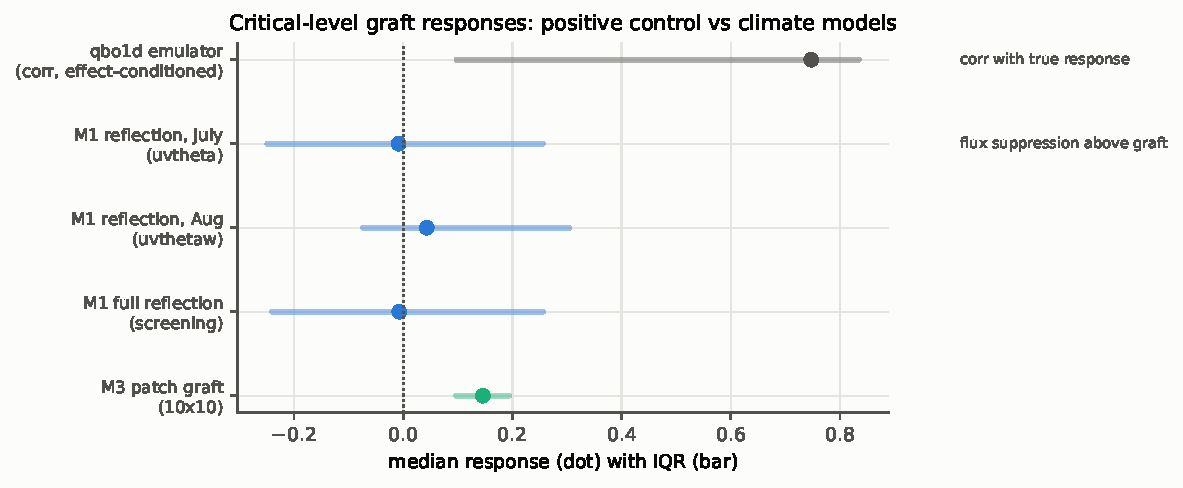
\includegraphics[width=\columnwidth]{figures/fig6_graft_battery.pdf}
\caption{Critical-level graft responses. The validated positive control responds strongly (top row: correlation with the true response, conditioned on detectable effect); the column models do not (suppression medians at zero); hotspot-center patch grafts elicit only weak partial-dose responses. Sources: \texttt{gateweek\_g1}, \texttt{d2\_battery}, \texttt{screen\_p\_grafts}.}
\label{fig:grafts}
\end{figure}

Findings: (i)~\emph{typical columns show no filtering response} (median suppression $-0.008$, $n{=}289$, July uvtheta; $+0.043$, $n{=}284$, August uvthetaw---replicated across month and the released checkpoint/input-variant axis, which is confounded $n{=}2$); (ii)~\emph{amplitude response is non-monotone} (median $\rho=0.49$ in both variants; testbed 0.94); (iii)~\emph{drag ignores wind rotation} (alignment 0.22/0.23; mean angular error 74--77$^\circ$); (iv)~\emph{hotspot centers respond weakly and partially}: 10$\times$10-column patch reflections (January; 28 admissible patches) give median suppression 0.125 ($\Mthree$) vs.\ 0.092 (paired $\Mone$) at max applied dose (median $\beta$ 0.40; 20/28 ladders have only two distinct doses; dose direction mixed---$\Mone$ 22/28 positive-monotone, $\Mthree$ 16/28 with 12 anti-monotone). This is far short of the near-complete flux removal linear theory prescribes at a full critical level, though per-patch quantitative expectations are not derived here (Sec.~\ref{sec:limits}).

Internal evidence matches. No hidden layer carries linearly readable $N^2$ or Richardson number beyond raw inputs (negative selectivity at every depth against both controls); flux sign is barely decodable anywhere; the linear flux readout collapses after layer 1 and crystallizes in the last hidden layer (88\% of full-model skill at the sixth hidden layer vs.\ 63\% at the fifth)---consonant with the anchor's finding that last-two-layer fine-tuning suffices for transfer. Sparse autoencoders fail their pre-registered quantitative gates at both audited sites (codes remain dense, $L_0\ge 106$ at all sparsity penalties tried; feature-map spatial coherence does not beat a random-direction null). Finally, the three architectures share a failure floor: top-1\% errors co-occur at 38--53$\times$ chance (rank correlations 0.78--0.88), consistent with a common data-limited ceiling (ERA5's own unresolved GW fraction).

\subsection{Hellinger is gameable where ladders are not}\label{sec:hellinger}
Two constructive demonstrations: variance-matched $\Mtwo$ is physically absurd (variance ratio 11.9) yet achieves \emph{better} pooled Hellinger (0.048) than $\Mthree$ (0.075); rolled $\Mthree$ loses its variance calibration entirely while pooled Hellinger is unchanged ($0.0745\!\to\!0.0744$). Pooled histograms reward marginal shape, not calibration; ladders (Eq.~\ref{eq:ladder}) discriminate in both directions. We recommend ladders alongside---or instead of---pooled Hellinger for distributional evaluation of flux surrogates.

\section{Limitations}\label{sec:limits}
\textbf{Scale.} T42 coarse-grained fluxes; expected horizontal group displacements are largely sub-cell, so the propagation null may be resolution-conditional; conversely the position prior may be weaker for domains without fixed layouts. \textbf{Offline only}; no online/coupled claims \citep{pahlavan2024}. \textbf{One checkpoint per configuration}; the checkpoint/input-variant robustness axis is confounded ($n{=}2$); no seed ensembles exist. \textbf{Roll attribution is an upper bound} (position-code removal and off-manifold degradation are inseparable with one checkpoint); four independent observations tie the collapse to position (symmetric distance curve; localization with exact identity control; hotspot concentration; $\Mone/\Mtwo$ controls; unchanged Hellinger). \textbf{Graft validity}: grafts break physical balance by design; admissibility and partial dosing bound but do not eliminate off-manifold effects; the positive control is 1D and column-local, covers the column-model arms (amplitude unconditionally; reflection under effect-detectability conditioning impossible in ERA5), and does \emph{not} cover the U-Net patch arm---whose weak-response result is therefore bounded/descriptive; per-patch linear-theory expectations are future work with the released ray tracer. \textbf{Dose caps}: median applied $\beta$ 0.40; 20/28 two-point ladders. \textbf{Labels}: ERA5's unresolved GW fraction bounds achievable physics (cf.\ the shared failure floor). \textbf{Epoch selection}: released epochs were presumably selected on 2015 validation loss; both audit months lie in 2015.

\section{Conclusion}\label{sec:conclusion}
Audited mechanistically, the celebrated nonlocality of a released neural GW parameterization hierarchy resolves into a genuine but isotropic, regime-reading use of long-range context; a variance-calibration advantage carried substantially by an implicit, padding-derived geographic prior; and an absence of the causal wave physics the skill is often taken to imply---established with a positive-controlled intervention battery inside a pre-registered funnel in which most of our own hypotheses, including the flagship, died. None of this diminishes in-distribution utility; it sharpens what the skill \emph{is}, how to measure it (ladders, not pooled Hellinger), which artifacts to fix (periodic padding; normalization metadata), and how much trust to extend where climate questions live: out of distribution.

\section*{Impact Statement}
This work audits, rather than deploys, ML climate surrogates. Its findings support more trustworthy use of such models by identifying artifacts and evaluation blind spots, and its released tooling (conversion utilities, audit protocols) lowers the cost of similar audits. We see no direct negative societal impact; misreading our bounded negatives as a blanket claim against ML parameterization would be a misuse we explicitly disclaim (Secs.~\ref{sec:intro},~\ref{sec:limits}).

\begin{thebibliography}{30}\small
\bibitem[Craig et al.(2026)]{craig2026} Craig, et al. Representational similarity across weather foundation models. \emph{arXiv:2605.23778}, 2026.
\bibitem[Espinosa et al.(2022)]{espinosa2022} Espinosa, Z.~I., Sheshadri, A., et al. Machine learning gravity wave parameterization generalizes to capture the QBO and response to increased CO$_2$. \emph{Geophys.\ Res.\ Lett.}, 49(8):e2022GL098174, 2022.
\bibitem[Fritts \& Alexander(2003)]{fritts2003} Fritts, D.~C. and Alexander, M.~J. Gravity wave dynamics and effects in the middle atmosphere. \emph{Rev.\ Geophys.}, 41(1):1003, 2003.
\bibitem[Gupta et al.(2024a)]{gupta2024ml} Gupta, A., et al. Machine learning global simulation of nonlocal gravity wave propagation. \emph{arXiv:2406.14775}, 2024.
\bibitem[Gupta et al.(2024b)]{gupta2024data} Gupta, A., Sheshadri, A., and Anantharaj, V. Gravity wave momentum fluxes from 1\,km global ECMWF Integrated Forecast System. \emph{Sci.\ Data}, 11, 2024. doi:10.1038/s41597-024-03699-x.
\bibitem[Gupta et al.(2025a)]{gupta2025} Gupta, A., Sheshadri, A., Roy, S., and Anantharaj, V. Offline performance of a nonlocal deep learning parameterization for climate model representation of atmospheric gravity waves. \emph{J.\ Adv.\ Model.\ Earth Syst.}, 17(10):e2025MS004977, 2025.
\bibitem[Gupta et al.(2025b)]{gupta2025prithvi} Gupta, A., et al. Finetuning AI foundation models to develop subgrid-scale parameterizations. \emph{arXiv:2509.03816}, 2025.
\bibitem[Hardiman et al.(2023)]{hardiman2023} Hardiman, S.~C., et al. Machine learning for nonorographic gravity waves in a climate model. \emph{Artif.\ Intell.\ Earth Syst.}, 2(4), 2023.
\bibitem[Haslauer et al.(2026)]{haslauer2026} Haslauer, K., et al. Explaining a U-Net parameterization of orographic gravity-wave fluxes with SHAP. \emph{arXiv:2605.05052}, 2026.
\bibitem[Islam et al.(2020)]{islam2020} Islam, M.~A., Jia, S., and Bruce, N.~D.~B. How much position information do convolutional neural networks encode? \emph{ICLR}, 2020.
\bibitem[Kayhan \& van Gemert(2020)]{kayhan2020} Kayhan, O.~S. and van Gemert, J.~C. On translation invariance in CNNs: Convolutional layers can exploit absolute spatial location. \emph{CVPR}, 2020.
\bibitem[MacMillan \& Ouellette(2025)]{macmillan2025} MacMillan, R. and Ouellette, J. Sparse autoencoders and causal steering in GraphCast. \emph{arXiv:2512.24440}, 2025.
\bibitem[Pahlavan et al.(2024)]{pahlavan2024} Pahlavan, H.~A., Hassanzadeh, P., and Alexander, M.~J. Explainable offline--online training of neural networks for parameterizations: A 1D gravity wave--QBO testbed in the small-data regime. \emph{Geophys.\ Res.\ Lett.}, 51(2), 2024.
\bibitem[Pahlavan et al.(2025)]{pahlavan2025} Pahlavan, H.~A., et al. Nonlocality of deep-learning parameterizations: receptive fields of CNN, FNO and MLP emulators. \emph{Geophys.\ Res.\ Lett.}, 2025. doi:10.1029/2024GL114136.
\bibitem[Richards \& Balan(2025)]{richards2025} Richards, C. and Balan, T. Linear probes in the Aurora weather model. \emph{arXiv:2511.07787}, 2025.
\bibitem[Rosenfeld \& Sonnewald(2026)]{rosenfeld2026} Rosenfeld, D. and Sonnewald, M. Physically grounded sparse probing of the Walrus foundation model. \emph{arXiv:2606.11657}, 2026.
\bibitem[Wang et al.(2022)]{wang2022} Wang, P., Yuval, J., and O'Gorman, P.~A. Non-local parameterization of atmospheric subgrid processes with neural networks. \emph{J.\ Adv.\ Model.\ Earth Syst.}, 14(10):e2022MS002984, 2022.
\end{thebibliography}

\appendix
\onecolumn
\section{The Hypothesis Funnel}\label{app:funnel}
Thirty hypotheses; verdicts and one-line evidence below. Full falsifiable statements, pre-registered kill criteria (with post-critic threshold amendments), and stamped per-verdict numbers are in the released \texttt{HYPOTHESIS\_TABLE.md} and \texttt{results/}.

\small
\begin{longtable}{llp{9.2cm}}
\toprule
ID & Verdict & Evidence (one line) \\
\midrule
\endhead
N1 & pass & finest-gate spatial structure 35$\times$ / temporal sensitivity 20$\times$ a random-init control \\
I2 & pass & clamped neighborhood is worse than $\Mone$ (gap recovery $-0.70$); context is information \\
N3 & pass & flattening finest gate: $+4.3\%$ RMSE, decaying $+1.4/+0.3/+0.1\%$ with scale \\
P4 & pass & $\Mthree$-only boundary seam $+5.1\%$ (Jul) / $+5.05\%$ (Jan); moves with padding under roll \\
A5 & pass & calibration ladder splits hierarchy; all CIs disjoint (Table~\ref{tab:ladder}) \\
F3 & pass & tail ordering matches Hellinger ordering (shared evidence with A5) \\
I4 & pass & occlusion saturation median 4 cells; $>16$ for 4/20 targets \\
R3 & pass & regime code transfers across regions (AUC 0.72 vs.\ 0.40 rand-init) \\
R6 & pass & flux lens collapses after layer 1, crystallizes at last hidden layer (88\% of skill) \\
\addlinespace
A1 & kill & linear stencil closes $-47\%$ of the $\Mone{\to}\Mtwo$ gap \\
A2 & kill & shear concentration 1.38 $<$ 1.5 (July); spawned A2b \\
F2 & kill & hotspot-type improvement ratio 1.06 (uniform) \\
N2 & kill & finest gate vs.\ instantaneous flux $r=-0.015$; below climatology null \\
I1 & kill & neighbor-ablation octant spread/mean 0.165 $<$ 0.20 \\
A4 & kill & clamp-delta top-5 PCs 23\%; projection moves 2.8\% toward $\Mone$ \\
N5 & kill & \emph{flagship}: influence isotropy 1.07 $<$ 1.3; wind alignment 9/20 \\
R1 & kill & $N^2$/Ri probe selectivity negative at every depth \\
R2 & kill & encoder reads $z_s$ at $R^2$ 0.06 vs.\ raw-input 0.45 (selectivity $-0.39$) \\
R5 & kill & no sign-vs-magnitude decodability separation (sign selectivity $\le$0.02) \\
P1 & kill & suppression above grafted reversal $-0.007$ (median, $n{=}277$) \\
P2 & kill & drag-rotation alignment 0.22; mean angular error 77$^\circ$ \\
P3 & kill & amplitude response median $\rho=0.49$; only 26\% monotone \\
I3 & kill & gradient features close 9.6\% of the gap (3 seeds: 0.085--0.106) \\
R4 & kill & SAE codes dense ($L_0\ge106$ at all $\lambda$); spatial coherence below random-direction null \\
\addlinespace
F1 & measured & top-1\% errors co-occur at 38--53$\times$ chance; rank corr.\ 0.78--0.88 \\
\addlinespace
A3 & deferred & reduced-scale retraining exceeded screening budget; causal half covered by N3 \\
N4 & deferred & conditional on N1 + an input-displacement null within budget \\
L1 & deferred & transfer-learning checkpoints not verifiable within scope \\
L2 & deferred & as L1 \\
A2b & killed at confirmation & January shear concentration 1.77 $<$ 2.0 (pattern reported descriptively) \\
\bottomrule
\end{longtable}

\section{Reproducibility}\label{app:repro}
All experiments are config-driven and seeded; every results file embeds its config hash, seed, and library versions. Released: the hypothesis table with pre-registered criteria; the append-only research log (including failures, logged deviations, and three adversarial critic reports); the WxC normalization conversion utilities and their validation tests; physics baselines with 14 analytic unit tests (39 passing tests overall); \texttt{make reproduce-figures}. Only released artifacts (checkpoints, code, public data) are used. Compute: a single CPU laptop (i7-1065G7); the entire audit is reproducible without a GPU.

\end{document}
